
\begin{frame}
\begin{small}
\frametitle{\centering  1-slide summary}
\begin{block}{Related second-order methods}
\begin{tabular}{c|c|c}
\toprule
\multirow{2}{*}{(Spall 2000)\footnotemark[1]} & Second-order SPSA & \multirow{2}{*}{\alert{4} simulations/iteration}\\
&  (\alert{2SPSA}) & \\\midrule
(Spall 2009)\footnotemark[2] & 2SPSA + feedback & \alert{4} simulations/iteration\\
\midrule
(Prashanth L.A. & Second-order RDSA & \multirow{2}{*}{\alert{3} simulations/iteration}\\
 et al 2016)\footnotemark[3] & (\alert{2RDSA})&\\
\bottomrule
\end{tabular}
\end{block}

\begin{block}{Our work}
We propose feedback and weighting mechanisms for improving Hessian estimate for 2RDSA algorithm.\\[4ex]
\end{block}

\footnotetext[1]{\tiny J.~C. Spall (2000), ``Adaptive stochastic approximation by the simultaneous
  perturbation method,'' \emph{IEEE TAC}.}
\footnotetext[2]{\tiny J.~C. Spall (2009), ``Feedback and weighting mechanisms for improving {Jacobian}
  estimates in the adaptive simultaneous perturbation algorithm,'' \emph{IEEE TAC}.}  
\footnotetext[3]{\tiny  Prashanth L.~A. et al. (2016) ``Adaptive system
  optimization using random directions stochastic approximation,'' \emph{IEEE TAC}.}
\end{small}
\end{frame}

%\begin{frame}
%\frametitle{\centering  Newton algorithm}
%\begin{block}{Stochastic version of Newton method}
%\begin{align}
%\label{eq:newton}
%\theta_{n+1} = \theta_n - a_n (\overline H_n)^{-1}\widehat\nabla f(\theta_n), 
%\end{align}
%\begin{itemize}
%\item $\widehat\nabla f(\theta_n)$ and $\overline H_n$ are estimates of the gradient and Hessian.
%\end{itemize}
%\end{block}
%\end{frame}

%\begin{frame}
%\begin{small}
%\frametitle{\centering  Newton RDSA}
%\begin{block}{2 RDSA}
%\begin{align}
%\label{eq:2rdsa}
%\theta_{n+1} = \theta_n - a_n \Upsilon(\overline H_n)^{-1}\widehat\nabla f(\theta_n), \\
%\overline H_n = \frac{n}{n+1} \overline H_{n-1} + \frac{1}{n+1} \widehat H_n.\label{eq:2rdsa-H}
%\end{align}
%\begin{itemize}
% \item $\widehat H_n$ is an estimate of the true Hessian. 
% \item $\overline H_n$ is a smoothed version of $\widehat H_n$. 
% \item $\Upsilon$ projects a matrix onto the set of positive definite matrices. 
%\end{itemize}
%
%\end{block}
%\end{small}
%\end{frame}

%\begin{frame}
%\begin{small}
%\frametitle{\centering  2RDSA Hessian estimate}
%\begin{block}{Function measurements}
%$y_{n}^+ = f(\theta_n+\delta_n d_n) + \xi_{n}^+,\quad y_{n}^- = f(\theta_n-\delta_n d_n) + \xi_{n}^-,\quad y_{n} = f(\theta_n) + \xi_{n}$
%\end{block}
%\begin{block}{}
%\begin{align}
%\label{eq:2rdsa-estimate-ber}
%\widehat H_n = M_n \left(\dfrac{y_n^+ + y_n^- - 2 y_n}{\delta_n^2}\right), \text{ where }\\
%& M_n =
%\left[
%\begin{array}{ccc}
%\frac{1}{\kappa}\left((d_n^1)^2\!-(1+\epsilon)\right) & \cdots & \frac{1}{2(1+\epsilon)^2}d_n^1 d_n^N\\
%\frac{1}{2(1+\epsilon)^2}d_n^2 d_n^1  &  \cdots & \frac{1}{2(1+\epsilon)^2}d_n^2 d_n^N\\
%\cdots&\cdots&\cdots\\
%\frac{1}{2(1+\epsilon)^2}d_n^N d_n^1 & \cdots &  \frac{1}{\kappa}\left((d_n^N)^2-(1+\epsilon)\right) \\
%\end{array}
%\right],\nonumber
%\end{align}
%where $\kappa = \tau \left(1- \dfrac{(1+\epsilon)^2}{\tau}\right)$ and $\tau = E (d_n^i)^4= \dfrac{(1+\epsilon)(1+(1+\epsilon)^3)}{(2+\epsilon)}$, for any $i=1,\ldots,N$. 
%\end{block}
%%\begin{columns}[T]
%%\begin{column}{.48\textwidth}
%%\color{red}\rule{\linewidth}{4pt}
%%Asymmetric Bernoulli
%%\begin{align}
%%%\label{eq:grad-unif}
%%M_n =
%%\left[
%%\begin{array}{ccc}
%%\frac{1}{\kappa}\left((d_n^1)^2\!-(1+\epsilon)\right) & \cdots & \frac{1}{2(1+\epsilon)^2}d_n^1 d_n^N\\
%%\frac{1}{2(1+\epsilon)^2}d_n^2 d_n^1  &  \cdots & \frac{1}{2(1+\epsilon)^2}d_n^2 d_n^N\\
%%\cdots&\cdots&\cdots\\
%%\frac{1}{2(1+\epsilon)^2}d_n^N d_n^1 & \cdots &  \frac{1}{\kappa}\left((d_n^N)^2-(1+\epsilon)\right) \\
%%\end{array}
%%\right],\nonumber
%%\end{align}
%%%\begin{equation}
%%%\label{eq:det-proj}
%%% d_n^i =
%%%  \begin{cases}
%%%   -1 &  \text{ w.p. } \dfrac{(1+\epsilon)}{(2+\epsilon)}, \\
%%%   1+\epsilon &  \text{ w.p. } \dfrac{1}{(2+\epsilon)},
%%%  \end{cases}
%%%\end{equation}
%%\end{column}
%%\begin{column}{.48\textwidth}
%%\color{blue}\rule{\linewidth}{4pt}
%%Uniform perturbations
%%\begin{align}
%%%\label{eq:grad-unif}
%%M_n =
%%\dfrac{9}{2\eta^4}\left[
%%\begin{array}{cccc}
%%\frac{5}{2}\left((d_n^1)^2-\frac{\eta^2}{3}\right) & \cdots & d_n^1 d_n^N\\
%%d_n^2 d_n^1  &  \cdots & d_n^2 d_n^N\\
%%\cdots&\cdots&\cdots\\
%%d_n^N d_n^1 & \cdots &  \frac{5}{2}\left((d_n^N)^2-\frac{\eta^2}{3}\right) \\
%%\end{array}
%%\right].\nonumber
%%\end{align}
%%%\begin{equation}
%%%\label{eq:det-proj-unif}
%%% d_n^i = Unif[-\eta,\eta], \eta>0.
%%% \end{equation}
%%\end{column}
%%\end{columns}
%\end{small}
%\end{frame}

\section{Random directions stochastic approximation (RDSA) + improved Hessian estimation}

\begin{frame}
\begin{small}
\frametitle{\centering Our algorithm}
\tikzstyle{na} = [baseline=-.5ex]
%\begin{block}{2 RDSA - IH}
\begin{itemize}
     \item Matrix projection 
         \tikz[na]\node [coordinate] (nL) {};
    \item Gradient estimate 
        \tikz[na]\node [coordinate] (nL1) {};
   \end{itemize}
   
\begin{equation}
\label{eq:e2rdsa}
\theta_{n+1} =   \theta_{n} - a_{n} 
\tikz[baseline]{\node[fill=blue!20,anchor=base] (tL) {$\Upsilon$};} 
(\overline H_{n})^{-1}\tikz[baseline]{\node[fill=green!20,anchor=base] (tL1) {$\widehat\nabla f(\theta_{n})$};}, 
\end{equation}

\begin{tikzpicture}[overlay]
%        \path[->]<1-> (nCPP) edge [bend left] (tCPP);
         \path[->] (nL) edge [bend left] (tL);
        \path[->] (nL1) edge [bend left] (tL1);
      
\end{tikzpicture}
\pause
\begin{equation}
\overline H_{n} =   (1-\tikz[baseline]{ \node[fill=green!60,anchor=base] (t3){$b_{n}$};})  \overline H_{n-1} + 
\tikz[baseline]{ \node[fill=green!60,anchor=base] (t3){$b_{n}$};} 
( 
\tikz[baseline]{ \node[fill=magenta!20,anchor=base] (tPPP1){$\widehat H_n$};} 
- 
\tikz[baseline]{\node[fill=red!60,anchor=base] (tPPP) {$\widehat \Psi_n$};}
),\label{eq:2rdsa-H}
\end{equation}
   \begin{itemize}
   \item Optimal step-sizes
        \tikz[na]\node [coordinate] (n3) {};

            \item Hessian estimate
        \tikz[na]\node [coordinate] (nPPP1) {};

    \item Feedback term
        \tikz[na]\node [coordinate] (nPPP) {};
    
\end{itemize}

\begin{tikzpicture}[overlay]
%        \path[->]<1-> (nCPP) edge [bend left] (tCPP);
                \path[->] (n3) edge [out=0, in=-90] (t3);
        \path[->] (nPPP1) edge [out=0, in=-90] (tPPP1);
        \path[->] (nPPP) edge [out=0, in=-90] (tPPP);
\end{tikzpicture}

%\begin{inparaenum}[\bfseries (i)]
%\item  $\widehat \Psi_n$ is a zero-mean feedback term that reduces the error in Hessian estimate; and\\
%\item $b_n$ is a general step-size that we optimize to improve the Hessian estimate.
%\end{inparaenum}
%\end{block}
\end{small}
\end{frame}

\begin{frame}{Overall flow of 2RDSA-IH}
%  \begin{figure}
% \centering
\tikzstyle{block} = [draw, fill=white, rectangle,
   minimum height=5em, minimum width=6em]
\tikzstyle{sum} = [draw, fill=white, circle, node distance=1cm]
\tikzstyle{input} = [coordinate]
\tikzstyle{output} = [coordinate]
\tikzstyle{pinstyle} = [pin edge={to-,thin,black}]

\begin{center}
 \scalebox{0.6}{\begin{tikzpicture}[auto, node distance=2cm,>=latex']
% We start by placing the blocks
\node (theta) at (-10,0) {$\bm{\theta_n}$};
\node [block, fill=blue!20,right=2cm of theta,label=below:{\color{bleu2}\bf Simulation},align=center] (sample) {\textbf{Using parameters }\\
$\bm{\theta_n, \theta_n \pm \delta_n d_n}$}; 
\node [block, fill=green!20,above right=3cm of sample,label=above:{\color{darkgreen!90}\bf Gradient estimation},align=center] (obj) {\textbf{Estimate} $\bm{\nabla f(\theta_{n})}$};
\node [block, fill=green!20,right=2cm of sample,label=above:{\color{darkgreen!90}\bf Hessian Estimation},align=center] (estcvar) {\textbf{Estimate} $\bm{\nabla^2 f(\theta_{n})}$};
\node [block, fill=green!20,below right=3cm of sample,label=below:{\color{darkgreen!90}\bf Improved Hessian estimate},align=center] (cvar) {\textbf{Feedback }\\ $\bm{\widehat \Psi_n}$};
\node [block, fill=red!20,right=8cm of sample, minimum height=8em,label=below:{\color{violet!90}\bf Gradient descent},align=center] (update) {\textbf{Update} $\bm{\theta_n}$};
\node [right=2cm of update] (end) {$\bm{\mathbf{\theta_{n+1}}}$};
\draw [thick,-triangle 45] (theta) --  (sample);
\draw [thick,-triangle 45] (sample) -- (obj);
\draw [thick,-triangle 45] (sample) -- (estcvar);
\draw [thick,-triangle 45] (sample) -- (cvar);
\draw [thick,-triangle 45] (obj) -- (update);
\draw [thick,-triangle 45] (estcvar) -- (update);
\draw [thick,-triangle 45] (cvar) -- (update);
\draw [thick,-triangle 45] (estcvar) -- (cvar);
\draw [thick,-triangle 45] (update) -- (end);
\end{tikzpicture}}
\end{center}
% \caption{Overall flow of 2RDSA-IH}
% \label{fig:algorithm-flow}
% \end{figure}
\end{frame}

% \section{Random directions stochastic approximation (RDSA)}
\begin{frame}
\begin{small}
\frametitle{\centering  RDSA gradient estimate}

\begin{block}{\alert{Function measurements}}
$y_{n}^+ = f(\tikz[baseline]{\node[fill=blue!20,anchor=base] (tL) {$\theta_n+\delta_n d_n$};} ) + \xi_{n}^+,\quad y_{n}^- = f(\tikz[baseline]{\node[fill=green!20,anchor=base] (tL1) {$\theta_n-\delta_n d_n$};}) + \xi_{n}^-$
\end{block}

\vspace{1.5ex}

\pause
\begin{block}{\alert{Gradient estimate}}
%\begin{columns}[T]
%\begin{column}{.48\textwidth}
%\color{red}\rule{\linewidth}{4pt}

\begin{align}
\label{eq:grad-unif}
\widehat\nabla f(\theta_n) = \frac{1}{1+\epsilon} d_n \left[ \dfrac{y_n^+ - y_n^-}{2\delta_n}\right].
\end{align}

Asymmetric Bernoulli distribution for $d_n^i, i=1,\ldots,N$:\\[1ex]
\begin{center}
\begin{tikzpicture}[thick]
  \node  at (0,0) [circle,draw=green!90,fill=green!80] (a1) {-1};
  \node  at (2,0) [circle,draw=green!90,fill=green!80] (a2) {$1+\epsilon$};
  \node at (-2, -1.5) (p1) {w.p. $\dfrac{1+\epsilon}{(2+\epsilon)}$};
  \node at (4, -1.5) (p2) {w.p. $\dfrac{1}{(2+\epsilon)}$};
  \draw (0.35,0) --  (1.4,0);
  \path[->] (p1.east) edge [out=0, in=-90] (a1);
  \path[->] (p2.west) edge [out=180, in=-90] (a2);
 \end{tikzpicture}
 \end{center}

%\end{column}
 
%\pause
%\begin{column}{.48\textwidth}
%\color{blue}\rule{\linewidth}{4pt}
%Uniform perturbations
%\begin{align}
%\label{eq:grad-unif}
%\widehat\nabla f(x_n) = \frac3{\eta^2} d_n \left[ \dfrac{y_n^+ - y_n^-}{2\delta_n}\right].
%\end{align}
%\begin{equation}
%\label{eq:det-proj-unif}
% d_n^i = Unif[-\eta,\eta], \eta>0.
% \end{equation}
%\end{column}
%\end{columns}
\end{block}
\end{small}
\end{frame}


\begin{frame} 
\begin{small}
\frametitle{\centering 2RDSA Hessian estimate}
\begin{block}{Function measurements}
$y_{n}^+ = f(\tikz[baseline]{\node[fill=blue!20,anchor=base] (tL) {$\theta_n+\delta_n d_n$};}) + \xi_{n}^+,\hspace{.16cm} y_{n}^- = f(\tikz[baseline]{\node[fill=green!20,anchor=base] (tL1) {$\theta_n-\delta_n d_n$};}) + \xi_{n}^-,\hspace{.16cm} y_{n} = f(\tikz[baseline]{\node[fill=red!20,anchor=base] (tL2) {$\theta_n$};}) + \xi_{n}$
\end{block}
\pause
\begin{block}{Hessian estimate $\widehat H_n$}
\begin{align}
\widehat H_n & = M_n \left(\dfrac{y_n^+ + y_n^- - 2 y_n}{\delta_n^2}\right) \nonumber \\
& =  M_n \left[\left(\dfrac{f(\theta_n+\delta_n d_n) + f(\theta_n-\delta_n d_n) - 2 f(\theta_n)}{\delta_n^2}\right) \right.\nonumber \\&\hspace{10em}+\left. \left(\dfrac{\xi_n^+ + \xi_n^- - 2 \xi_n}{\delta_n^2}\right)\right] \nonumber \\
& = 
M_n \left(\tikz[baseline]{\node[fill=red!20,anchor=base] (tL1) {$d_n\tr \nabla^2 f(\theta_n) d_n$};} +  O(\delta_n^2) + \tikz[baseline]{\node[fill=blue!20,anchor=base] (tL2) {$\left(\dfrac{\xi_n^+ + \xi_n^- - 2 \xi_n}{\delta_n^2} \right)$};}\right).\label{eq:h0}
\end{align}

\hspace{-2em}    Want to recover\\ $\nabla^2 f(\theta_n)$ from this \tikz[na]\node [coordinate] (nL1) {};
    \hspace{3cm}  Zero-mean \tikz[na]\node [coordinate] (nL2) {}; 
\begin{tikzpicture}[overlay]
         \path[->] (nL1) edge [out=0, in=-90] (tL1);
        \path[->] (nL2) edge [out=0, in=-90] (tL2);
\end{tikzpicture}
\end{block}
\end{small}
\end{frame}


\begin{frame}
\begin{small}
\frametitle{\centering  How to choose $M_n$?}
\begin{block}{Asymmetric Bernoulli Perturbation}
\begin{align}
\label{eq:2rdsa-estimate-ber}
 M_n =
\left[
\begin{array}{ccc}
\frac{1}{\kappa}\left((d_n^1)^2\!-(1+\epsilon)\right) & \cdots & \frac{1}{2(1+\epsilon)^2}d_n^1 d_n^N\\
\frac{1}{2(1+\epsilon)^2}d_n^2 d_n^1  &  \cdots & \frac{1}{2(1+\epsilon)^2}d_n^2 d_n^N\\
\cdots&\cdots&\cdots\\
\frac{1}{2(1+\epsilon)^2}d_n^N d_n^1 & \cdots &  \frac{1}{\kappa}\left((d_n^N)^2-(1+\epsilon)\right) \\
\end{array}
\right],
\end{align}
where $\kappa = \tau \left(1- \dfrac{(1+\epsilon)^2}{\tau}\right)$ and $\tau = E (d_n^i)^4= \dfrac{(1+\epsilon)(1+(1+\epsilon)^3)}{(2+\epsilon)}$, for any $i=1,\ldots,N$. 
\end{block}
%\pause
%\begin{block}{Uniform perturbations}
%\begin{align}
%\label{eq:2rdsa-estimate-unif}
%M_n =
%\dfrac{9}{2\eta^4}\left[
%\begin{array}{cccc}
%\frac{5}{2}\left((d_n^1)^2-\frac{\eta^2}{3}\right) & \cdots & d_n^1 d_n^N\\
%d_n^2 d_n^1  &  \cdots & d_n^2 d_n^N\\
%\cdots&\cdots&\cdots\\
%d_n^N d_n^1 & \cdots &  \frac{5}{2}\left((d_n^N)^2-\frac{\eta^2}{3}\right) \\
%\end{array}
%\right].
%\end{align}
%\end{block}

\end{small}
\end{frame}

%\begin{frame}
%\begin{small}
%\frametitle{\centering  2RDSA Hessian estimate}
%\begin{block}{Uniform perturbations}
%\begin{align}
%\label{eq:2rdsa-estimate-unif}
%M_n =
%\dfrac{9}{2\eta^4}\left[
%\begin{array}{cccc}
%\frac{5}{2}\left((d_n^1)^2-\frac{\eta^2}{3}\right) & \cdots & d_n^1 d_n^N\\
%d_n^2 d_n^1  &  \cdots & d_n^2 d_n^N\\
%\cdots&\cdots&\cdots\\
%d_n^N d_n^1 & \cdots &  \frac{5}{2}\left((d_n^N)^2-\frac{\eta^2}{3}\right) \\
%\end{array}
%\right].
%\end{align}
%\end{block}
%\end{small}
%\end{frame}




\begin{frame}
\begin{small}
\frametitle{\centering Zero-mean feedback term}
\tikzstyle{na} = [baseline=-.5ex]
 \textcolor{red!60}{Zero-mean term}\tikz[na]\node [coordinate] (n1) {};
 \begin{block}{\alert{Mean of the  Hessian estimate}}
\begin{align}
 \E\left[\left.\widehat H_n\right| \F_n\right] = & \nabla^2 f(\theta_n) + \tikz[baseline]{ \node[fill=red!60,anchor=base] (t1){$\E\left[\left.\Psi_{n}(\nabla^2 f(\theta_n))\right| \F_n\right]$};}  +  O(\delta_n^2)\nonumber\\
&+\E\left[\left.\left(\dfrac{\xi_n^+ + \xi_n^- - 2 \xi_n}{\delta_n^2} \right)\right| \F_n\right], \label{eq:hnhat}
\end{align}
\end{block}
\begin{tikzpicture}[overlay]
        \path[->]<1-> (n1) edge [bend left] (t1);   
\end{tikzpicture}
\pause
\begin{block}{\alert{Feedback term}}
\begin{align}
\Psi_{n}(H) =  [M_n]_{D}\left(d_{n}\tr \, [H]_{N} \, d_{n}\right) +  [M_n]_{N}\left(d_{n}\tr \, [H]_{D} \, d_{n}\right).\label{eq:psi}
\end{align}
\end{block}
\footnotetext[1]{\tiny For any matrix $P$, $[P]_{D}$ refers to a matrix that retains only the diagonal entries of $P$ and replaces all the remaining  entries with zero.}
\footnotetext[2]{\tiny $[P]_{N}$ to refer to a matrix that retains only the off-diagonal entries of $P$, while replaces all the diagonal entries with zero.}
\end{small}
\end{frame}

\begin{frame}
\begin{small}
\frametitle{\centering Zero-mean feedback term}
\begin{block}{\alert{Problem}}
Feedback term is function of current Hessian  $\nabla^2 f$.
\end{block}
\pause
\begin{block}{\alert{Solution}}
Use $\overline H_{n-1}$ as a proxy for $\nabla^2 f$.
\begin{align}
\widehat \Psi_n = \Psi_{n} (\tikz[baseline]{ \node[fill=red!60,anchor=base] (t1){$\overline H_{n-1}$};}).
\label{eq:psinhat}
\end{align}
\end{block}
\end{small}
\end{frame}

\begin{frame}
\begin{small}
\frametitle{\centering Step-size optimization}
\begin{block}{\alert{Rewriting the Hessian recursion}}
\begin{align}
\label{eq:hess}
\overline H_n = \sum\limits_{i=0}^{n} \tilde b_k(\widehat H_i -\widehat \Psi_i).
\end{align}
\end{block}
\pause
\begin{block}{\alert{Optimization problem for weights}}
\begin{align}
\min_{ \{\tilde b_k\} } \sum \limits_{i=0}^{n} (\tilde b_k)^2 \delta_i^{-4}, \text{ subject to} \label{eq:wn-opt}\\
\tilde b_i \geq 0 ~\forall i \text{ and }\sum \limits_{i=0}^{n} \tilde b_i = 1.
\end{align}
\end{block}
\end{small}
\end{frame}

\begin{frame}
\begin{small}
\frametitle{\centering Step-size optimization}
\begin{block}{\alert{Above optimization problem solution}}
\begin{align}
\tilde b_i^* = \delta_i^{4}/\sum \limits_{j=0}^{n} \delta_j^{4}, i=1,\ldots,n.
\end{align}
\end{block}
\pause
\begin{block}{\alert{Optimal weights for original Hessian recursion}}
\begin{align}
\label{eq:wieghts}
b_i  = \delta_i^{4}/\sum\limits_{j=0}^{i} \delta_j^{4}.
\end{align}
\end{block}
\footnotetext[1]{Step-size optimization is a relatively straightforward migration from Spall 2009.}
\end{small}
\end{frame}

\begin{frame}
\begin{small}
\frametitle{\centering Convergence analysis}

\begin{lemma}(\alert{Bias in Hessian estimate})
\label{lemma:2rdsa-bias}
From Prashanth L.~A. et al. (2016)\footnotemark[1], we have a.s. that\footnotemark[2], for $i,j = 1,\ldots,N$,
\begin{align}
\left|\E\left[
\left. \widehat H_n(i,j) \right| \F_n \right] - \nabla^2_{ij} f(\theta_n)\right| = O(\delta_n^2).
\end{align} 
\end{lemma}
\begin{theorem}(\alert{Strong Convergence of Hessian})
\label{thm:2rdsa-H}
Under assumptions similar to those for 2SPSA and 2RDSA, we have that 
$$\theta_n \rightarrow \theta^*, \overline H_n \rightarrow \nabla^2 f(\theta^*) \text{ a.s. as } n\rightarrow \infty.$$ 
\end{theorem}
\footnotetext[1]{\tiny  Prashanth L.~A. et al. (2016) ``Adaptive system
  optimization using random directions stochastic approximation,'' \emph{IEEE TAC}.}
\footnotetext[2]{\tiny Here $\widehat H_n(i,j)$ and $\nabla^2_{ij}f(\cdot)$ denote the $(i,j)$th entry in the Hessian estimate $\widehat H_n$ and the true Hessian $\nabla^2 f(\cdot)$, respectively.}
\end{small}
\end{frame}


%\begin{frame}
%\begin{small}
%\frametitle{\centering Convergence analysis}
%\begin{theorem}(\textbf{Strong Convergence of Hessian})
%\label{thm:2rdsa-H}
%Under assumptions similar to those for 2SPSA and 2RDSA, we have that 
%$$\theta_n \rightarrow \theta^*, \overline H_n \rightarrow \nabla^2 f(\theta^*) \text{ a.s. as } n\rightarrow \infty.$$ 
%\end{theorem}
%\end{small}
%\end{frame}

\section{Numerical Results}
\begin{frame}
\begin{small}
\frametitle{\centering Numerical Results}
\begin{block}{\alert{Quadratic loss}}
\begin{align}
f(x) = \theta\tr A \theta + b\tr \theta.\label{eq:quadratic}
\end{align}
\end{block}
\begin{block}{\alert{Fourth-order loss}}
\begin{align} 
f(x) = \theta\tr A\tr A \theta + 0.1 \sum_{j=1}^N (A\theta)^3_j + 0.01 \sum_{j=1}^N (A\theta)^4_j.\label{eq:4thorder}
 \end{align} 
 \end{block}
 \end{small}
\end{frame}

\begin{frame}
\begin{small}
\frametitle{\centering Numerical Results}
\begin{block}{\alert{Normalized MSE (NMSE)} }
\begin{align}
\l \theta_{n_\text{end}} - \theta^* \r^2 / \l \theta_0 - \theta^*\r^2
\end{align}
\end{block}
\begin{block}{ \alert{Normalized loss}}
\begin{align} 
f(\theta_{n_\text{end}})/f(\theta_0)
 \end{align} 
 \end{block}
 \end{small}
\end{frame}


\begin{frame}
\begin{small}
\frametitle{}

\vspace{2ex}

\begin{table}
\centering
 \caption{Normalized loss values for fourth-order  objective \eqref{eq:4thorder} with noise: simulation budget = 10,000 and standard error from $500$ replications shown after $\pm$}
\label{tab:norloss-4thf}
\adjustbox{max height=\dimexpr\textheight-5.1cm\relax,
           max width=\textwidth}{
\begin{tabular}{|c|c|c|}
\toprule
\rowcolor{gray!20}
\multicolumn{3}{||c|}{\multirow{2}{*}{\textbf{Noise parameter $\sigma=0.1$}}}\\[1em]
%&&&\\
\midrule
  & \multirow{2}{*}{\textbf{Regular}} & \textbf{Improved Hessian}  \\
  & & \textbf{ estimation} \\
 \midrule
\textbf{2SPSA} & $0.132 \pm 0.0267$ & $0.104 \pm 0.0355$\\
&&\\
\textbf{2RDSA-Unif\footnotemark[1]} &$0.115 \pm 0.0214$ & $0.0271 \pm 0.0538$\\ 
&&\\
\textbf{2RDSA-AsymBer}& $0.0471 \pm 0.021$& $\bm{0.0099 \pm 0.0014}$\\
 \bottomrule
% \rowcolor{gray!20}
%\multicolumn{3}{||c|}{\multirow{2}{*}{\textbf{Noise parameter $\sigma=0$}}}\\[1em]
%%&&&\\
%\midrule
%  & \multirow{2}{*}{\textbf{Regular}} & \textbf{Improved Hessian}  \\
%  & & \textbf{ estimation} \\
% \midrule
%\textbf{2SPSA} & $0.0795 \pm 0.0234$ & $0.0628 \pm 0.0234$\\
%&&\\
%\textbf{2RDSA-Unif} &$0.0813 \pm 0.0275$ & $0.0214 \pm 0.00376$\\ 
%&&\\
%\textbf{2RDSA-AsymBer}& $0.0199 \pm 0.0114$& $\bm{0.0098 \pm 0.00147}$\\
% \bottomrule
 \end{tabular}}
\end{table}
\footnotetext[1]{2RDSA-Unif uses $Unif [-1,1]$ with a different $M_n$.}
 \end{small}
\end{frame}



\begin{frame}
\begin{small}
\frametitle{}

\vspace{2ex}

\begin{table}
\centering
 \caption{NMSE values for quadratic objective \eqref{eq:quadratic} with  noise: simulation budget = 10,000 and standard error from $500$ replications shown after $\pm$}
\label{tab:nmse-quadratic}
\adjustbox{max height=\dimexpr\textheight-5.1cm\relax,
           max width=\textwidth}{
\begin{tabular}{|c|c|c|}
\toprule
\rowcolor{gray!20}
\multicolumn{3}{||c|}{\multirow{2}{*}{\textbf{Noise parameter $\sigma=0.1$}}}\\[1em]
%&&&\\
\midrule
  & \multirow{2}{*}{\textbf{Regular}} & \textbf{Improved Hessian}  \\
  & & \textbf{ estimation} \\
 \midrule
\textbf{2SPSA} & $0.9491 \pm 0.0131$ & $0.5495 \pm 0.0217$\\
&&\\
\textbf{2RDSA-Unif} &$1.0073 \pm 0.0140$ & $0.1953 \pm 0.0095$\\ 
&&\\
\textbf{2RDSA-AsymBer}& $0.1667 \pm 0.0095$& $\bm{0.0324 \pm 0.0007}$\\
 \bottomrule
%\rowcolor{gray!20}
%\multicolumn{3}{||c|}{\multirow{2}{*}{\textbf{Noise parameter $\sigma=0$}}}\\[1em]
%%&&&\\
%\midrule
%  & \multirow{2}{*}{\textbf{Regular}} & \textbf{Improved Hessian}  \\
%  & & \textbf{ estimation} \\
% \midrule
%\textbf{2SPSA} & $0.7325 \pm 0.0180$ & $0.3939 \pm 0.0230$\\
%&&\\
%\textbf{2RDSA-Unif} &$0.9834 \pm 0.0170$ & $0.1623 \pm 0.0086$\\ 
%&&\\
%\textbf{2RDSA-AsymBer}& $0.0686 \pm 0.0078$& $\bm{0.0316 \pm 0.0006}$\\
% \bottomrule
\end{tabular}}
\end{table}
 \end{small}
\end{frame}

%\begin{frame}
%\frametitle{\centering Numerical Results}
%\newcommand{\errorband}[5][]{ % x column, y column, error column, optional argument for setting style of the area plot
%\pgfplotstableread[col sep=comma, skip first n=2]{#2}\datatable
%    % Lower bound (invisible plot)
%    \addplot [draw=none, stack plots=y, forget plot] table [
%        x={#3},
%        y expr=\thisrow{#4}-2*\thisrow{#5}
%    ] {\datatable};
%
%    % Stack twice the error, draw as area plot
%    \addplot [draw=none, fill=gray!40, stack plots=y, area legend, #1] table [
%        x={#3},
%        y expr=4*\thisrow{#5}
%    ] {\datatable} \closedcycle;
%
%    % Reset stack using invisible plot
%    \addplot [forget plot, stack plots=y,draw=none] table [x={#3}, y expr=-(\thisrow{#4}+2*\thisrow{#5})] {\datatable};
%}
%
% \begin{figure}
%    \centering
%\tabl{c}{\scalebox{0.9}{\begin{tikzpicture}
%      \begin{axis}[
%	xlabel={number of simulations},
%	ylabel={Normalized loss},
%       legend entries={
%	 ,2SPSA,,2SPSA-IH,,2RDSA-Unif,,2RDSA-Unif-IH,,2RDSA-AsymBer,,2RDSA-AsymBer-IH },
%        %legend pos=outer north east,
%			legend style={
%at={(0,0)},
%anchor=north,at={(axis description cs:0.5,-0.2)},legend columns=2}	]
%      % 2SPSA
%      \errorband[red!50!white, opacity=0.3]{norloss_vs_simulations_noisycase.csv}{0}{1}{2}
%      \addplot [thick, red,mark=square*,mark options={scale=0.7}] table [x index=0, y index=1,col sep=comma] {norloss_vs_simulations_noisycase.csv};
%			%%% With IH
%      % 2SPSA
%      \errorband[darkgray!50!white, opacity=0.3]{norloss_vs_simulations_noisycase.csv}{0}{7}{8}
%      \addplot [thick, darkgray,mark=*,mark options={scale=0.75}] table [x index=0, y index=7,col sep=comma] {norloss_vs_simulations_noisycase.csv};
%			
%      % 2RDSA-Unif
%      \errorband[blue!50!white, opacity=0.3]{norloss_vs_simulations_noisycase.csv}{0}{3}{4}
%      \addplot [thick, blue,mark=square*,mark options={scale=0.7}] table [x index=0, y index=3,col sep=comma] {norloss_vs_simulations_noisycase.csv};
%			%%% With IH
%      % 2RDSA-Unif
%      \errorband[magenta!50!white, opacity=0.3]{norloss_vs_simulations_noisycase.csv}{0}{9}{10}
%      \addplot [thick, magenta,mark=*,mark options={scale=0.75}] table [x index=0, y index=9,col sep=comma] {norloss_vs_simulations_noisycase.csv};
%
%
%      % 2RDSA-AsymBer
%      \errorband[green!50!white, opacity=0.3]{norloss_vs_simulations_noisycase.csv}{0}{5}{6}
%      \addplot [thick, darkgreen,mark=square*,mark options={scale=0.7}] table [x index=0, y index=5,col sep=comma] {norloss_vs_simulations_noisycase.csv};
%			%%% With IH	
%      % 2RDSA-AsymBer
%      \errorband[violet!50!white, opacity=0.3]{norloss_vs_simulations_noisycase.csv}{0}{11}{12}
%      \addplot [thick, violet, mark=*,mark options={scale=0.75}] table [x index=0, y index=11,col sep=comma] {norloss_vs_simulations_noisycase.csv};
%      \end{axis}
%      \end{tikzpicture}}\\}
%			\caption{Normalized loss vs. number of simulations for fourth-order loss \eqref{eq:4thorder} with $\sigma=0.1$ for 2SPSA, 2RDSA-Unif and 2RDSA-AsymBer algorithms with/without improved Hessian estimation: bands around the curves represent standard error from $500$ replications. }
%      \label{fig:norlossvssims} 
%\end{figure} 
%\end{frame}

























